\subsection{Concordia Contracts Migrator} \label{subsection:4-3-3-concordia-contracts-migrator}

\subsubsection{Περιγραφή - Στόχοι υπηρεσίας}

Η υπηρεσία αυτή αποτελείται από ένα εκτελέσιμο πρόγραμμα γραμμής εντολών βασισμένο στο άρθρωμα concordia-contracts που αναλύθηκε σε προηγούμενη υποενότητα (\ref{subsection:4-3-1-software-units}). Το πρόγραμμα, κατά την εκτέλεσή του, μεταγλωττίζει τα contracts και έπειτα τα μεταφορτώνει στο blockchain το οποίο είναι ορισμένο με χρήση μεταβλητών περιβάλλοντος. Τέλος, αν οι κατάλληλες μεταβλητές περιβάλλοντος είναι ορισμένες, το πρόγραμμα μεταφορτώνει τα τελικά artifacts σε αποθετήριο Concordia Contracts Provider. Η αρχιτεκτονική της υπηρεσίας φαίνεται στο παρακάτω σχήμα (σχήμα \ref{figure:4-3-concordia-contracts-migrator-architecture}).

\begin{figure}[H]
    \centering
    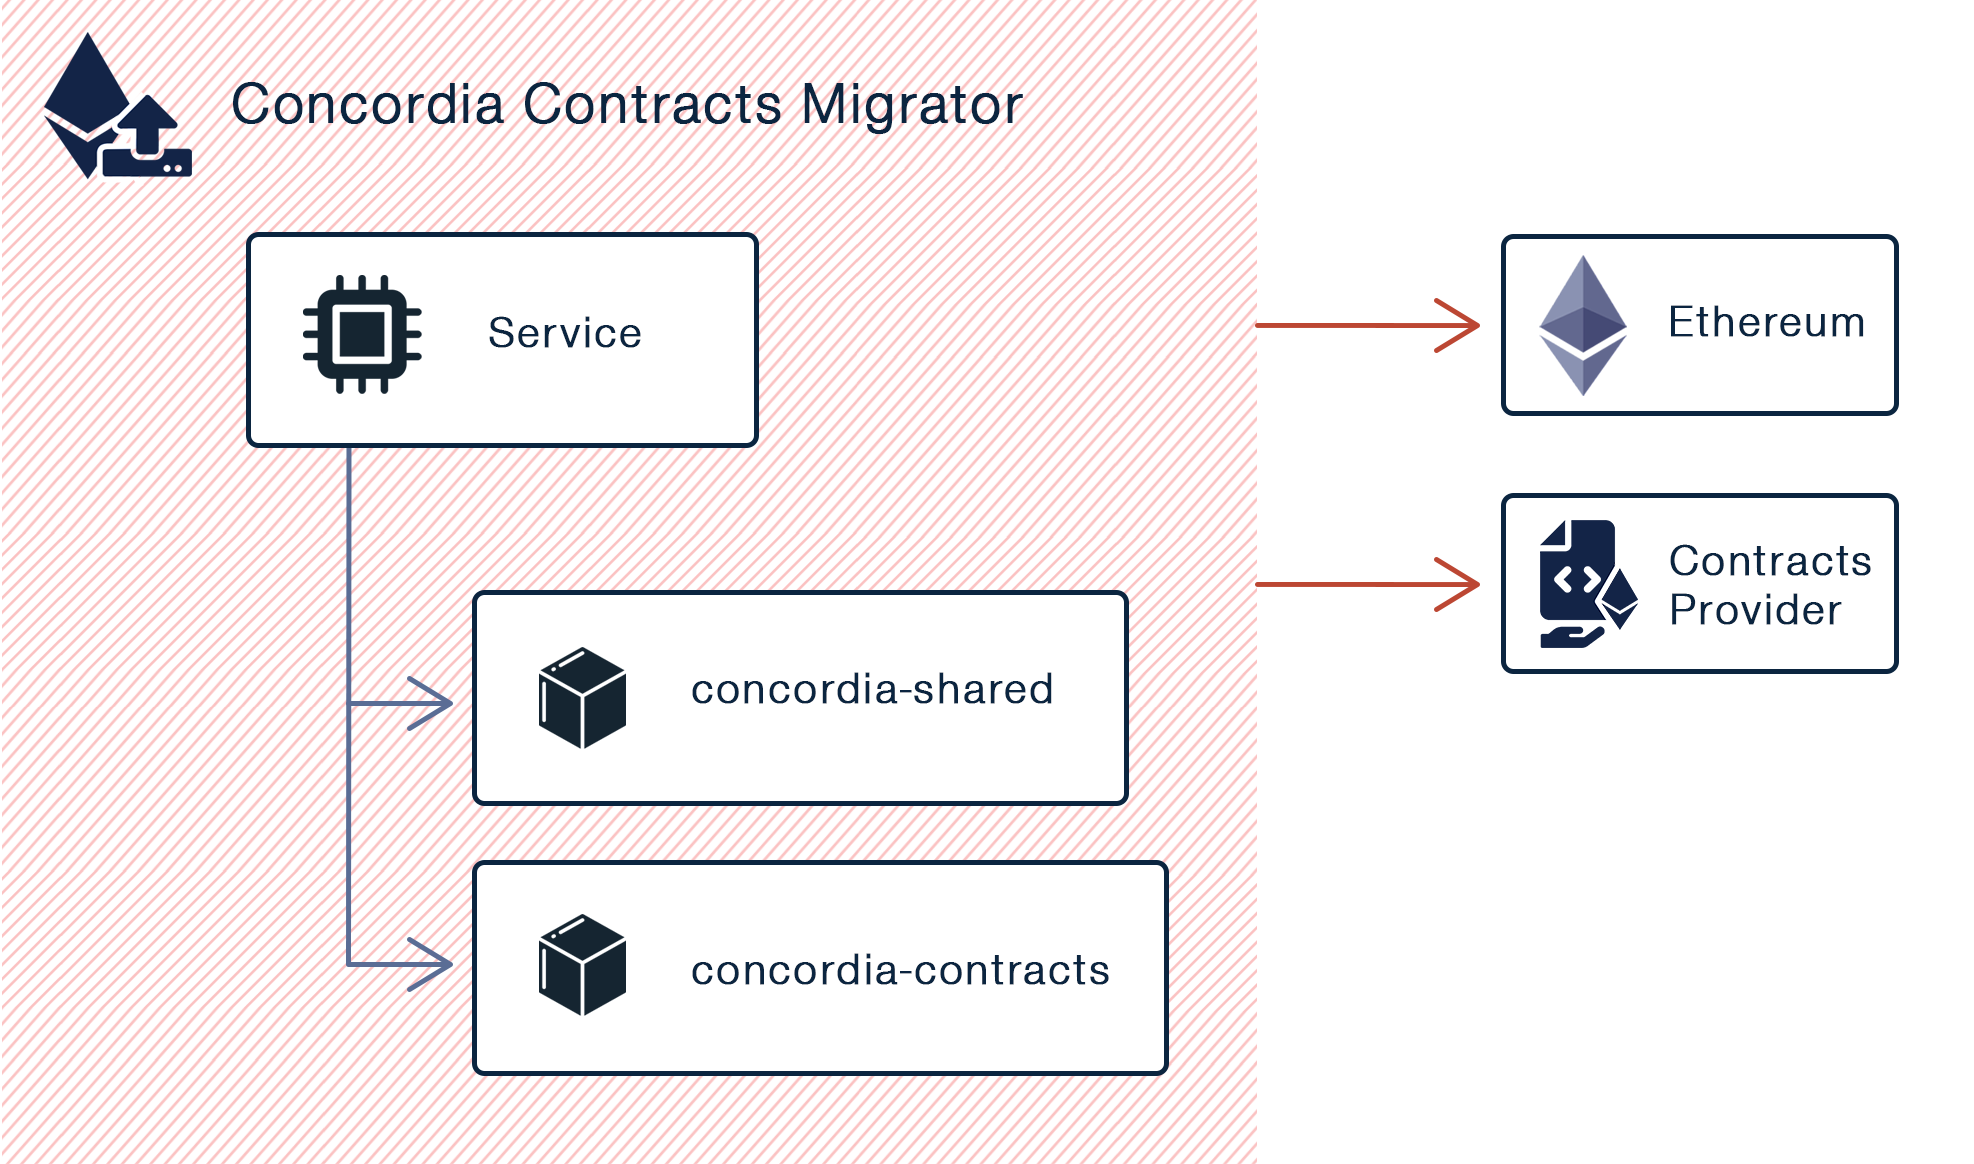
\includegraphics[width=.6\textwidth]{assets/figures/chapter-4/4.3.architecture-4.3.3.concordia-contracts-migrator-architecture.png}
    \caption{Αρχιτεκτονική υπηρεσίας Concordia Contracts Migrator}
    \label{figure:4-3-concordia-contracts-migrator-architecture}
\end{figure}

\subsubsection{Διανομή}

Η υπηρεσία αυτή γίνεται διαθέσιμη για χρήση ως docker image μέσω του αποθετηρίου εικόνων dockerhub. Οι χρήστες μπορούν χρησιμοποιώντας μεταβλητές περιβάλλοντος να αλλάξουν τη διεύθυνση του blockchain και την τοποθεσία της υπηρεσίας Contracts Provider στην οποία το πρόγραμμα θα μεταφορτώσει τα contracts και τα artifacts.